\documentclass{article}
\usepackage[usenames,dvipsnames]{pstricks}
\usepackage{amsfonts}
\usepackage{amsmath}
\usepackage{amssymb}
\usepackage{epsfig}
\usepackage{graphicx}
\usepackage{mathrsfs}
\usepackage{pst-grad} % For gradients
\usepackage{pst-plot} % For axes
\usepackage{subcaption}
\usepackage{tikz}

\title{COMP590: Homework 1}
\author{Professor Jason Isaacs}
\date{March 3, 2016}

\begin{document}
\maketitle
\section*{Problem 1}
By definition, each edge connects two vertices, and each vertex $v_i$ is in
exactly $\text{deg}(v_i)$ edges. From this, we see that the sum of the
degrees of each vertex in our graph will give us the number of edges in the
graph counted twice, once for each vertex in each edge. Thus for a graph
$\mathcal{G}$ with edges $E$ and vertices $V$. 
\[ \sum_{v_i \in V} v_i = 2|E| \]
or 
\[ \frac{\sum_{v_i \in V} v_i}{2} = |E| \]
as required.

From this we can see that the trace of the graph Laplacian is even. The trace of
the Laplacian is the sum of the degrees of each vertex, which we just showed was
twice the number of edges, which is a multiple of 2 and hence even. We know that
the trace of the Laplacian is the sum of the degrees of each vertex because 
\[ T(L) = T(\Delta - A) = T(\Delta) \]
because the adjacency matrix has a zero diagonal. 

The fact that the sum of the degrees of each vertex is even, implies that the
number of odd degree vertices is even because, as any middle schooler knows, the
sum of two even numbers and the sum of two odd numbers is even, but the sum of
an odd and an even number is odd. In other words, if the number of odd degree
vertices in a graph is odd, the sum of the graph's degrees would be odd, which
we just showed to be impossible. Thus the number of odd degree vertices is even.

\section*{Problem 2}
First off, note that the sum of the degree sequence
\[ 3, 3, 3, 3, 5, 6, 6, 6, 6, 6, 6 \]
is 53, which is odd. No graph can have an odd degree sum due to the formula from
problem 1. Thus no graph exists with this degree sequence.

For the second problem I used the Erd\H{o}s--–Gallai theorem, which I implemented in the
following MATLAB code taken from my ``\texttt{degree\_seq.m}'' file.
\begin{verbatim}
function [ exists ] = degree_seq( sequence )
%Implements the Erd?s?Gallai theorem
if( mod(sum(sequence),2) )
    exists = false;
    return
end
sorted_seq = sort(sequence,'descend');
for k = 1:length(sorted_seq)
    if( sum(sorted_seq(1:k)) > k*(k-1) + sum(min(k, sorted_seq(k+1:end))) )
        exists = false;
        return
    end
end
exists = true;
end
\end{verbatim}
This returns false, so I conclude that no graph exists. 

For more information on the Erd\H{o}s--–Gallai theorem, see 
\begin{verbatim}
https://en.wikipedia.org/wiki/Erd%C5%91s%E2%80%93Gallai_theorem
\end{verbatim}


\section*{Problem 3}
Let $\mathcal{G} = (E,V)$ be a graph with adjacency matrix $A_{\mathcal{G}}$,
and complement $\overline{\mathcal{G}} = (\overline{E}, V)$ and adjacency matrix
$A_{\overline{\mathcal{G}}}$. Then we can say that 
\[ \text{deg}_{\overline{\mathcal{G}}}(v_i) = (n-1) -
\text{deg}_{\mathcal{G}}(v_i), \forall v_i \in V \]
\[ \Delta_{\overline{\mathcal{G}}} = (n-1)I -
\Delta_{\mathcal{G}} \]
and
\[ A_{\overline{\mathcal{G}}} = \vec{1}\vec{1}^t - I - A_{\mathcal{G}} \]
where $n = |V|$ and $\vec{1}$ is the $n\times 1$ vector of all 1s. From this we
can conclude that
\[ L(\mathcal{G}) + L(\overline{\mathcal{G}}) = \Delta_{\mathcal{\overline{G}}} -
A_{\mathcal{\overline{G}}} + \Delta_{\mathcal{G}} - A_{\mathcal{G}} = nI - \vec{1}\vec{1}^t
\]
as required.

\section*{Problem 4}
I attach a full folder of related code snippets, but the meat of the code
(containing the algorithm) is below, taken from ``\texttt{Connected.m}''
\begin{verbatim}
function [ output_args ] = Connected( adjacency_matrix )
%Connected uses depth first search to determine if a graph is connected.
visited = zeros(length(adjacency_matrix),1);
to_visit = [ 1 ];
while ~isempty(to_visit);
    pos = to_visit(1);
    to_visit = to_visit(2:end);
    if(visited(pos))
        continue;
    end
    visited(pos) = 1;
    
    connects_to = find(adjacency_matrix(pos,:));
    for jj = connects_to
        if(~visited(jj))
            to_visit =  [jj to_visit];
        end
    end
end
output_args = isequal(length(adjacency_matrix),sum(visited));
\end{verbatim}
To invoke this, simply run the ``\texttt{Connected.m}'' file on the adjacency matrix. I
tested this using the eigenvalues of the Laplacian in
``\texttt{test\_connected.m}.'' I successfully used over 100,000 different graphs, of sizes
varying from 5 to 50.

\section*{Problem 5}
For this problem I used a 20 node graph with the following randomly generated
initial positions. As shown in the attached figures, the convergence time
increases uniformly with the addition of edges, and the second eigenvalue of the
Laplacian, which was shown in class to relate to convergence, increases
uniformly. However, not all added edges increase convergence equally. While all
additional edges increase convergence, the rate of increase seems to incur
diminishing marginal growth per edge on a node, resulting in the ``lumpy''
figures. Thus the figures would change if the edges were added in a different
order, and would be smoother if the edges were added in a more uniform manor.
See \texttt{hw1\_problem5.m}.

\begin{center}
\begin{tabular}{c|cc}
Node & $x$ position & $y$ position \\\hline
1 & 0.103180 & 0.196814\\
2 & 0.616154 & 0.836510\\
3 & 0.193730 & 0.911811\\
4 & 0.558131 & 0.099734\\
5 & 0.880397 & 0.987891\\
6 & 0.825086 & 0.952190\\
7 & 0.630737 & 0.357484\\
8 & 0.164353 & 0.428640\\
9 & 0.441313 & 0.660809\\
10 & 0.907688 & 0.103857\\
11 & 0.183725 & 0.184508\\
12 & 0.776641 & 0.892691\\
13 & 0.677526 & 0.853540\\
14 & 0.936871 & 0.227591\\
15 & 0.470356 & 0.927209\\
16 & 0.696634 & 0.228739\\
17 & 0.746190 & 0.301215\\
18 & 0.819661 & 0.751948\\
19 & 0.848511 & 0.684286\\
20 & 0.482299 & 0.097935
\end{tabular}
\end{center}

\begin{figure}[h!]
\caption{Convergence Time}
\centering
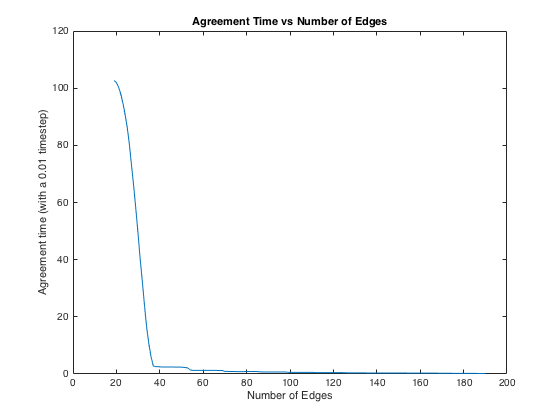
\includegraphics[width=\textwidth]{./Agreement_time-edges.png}
\end{figure}
\begin{figure}[h!]
\caption{Convergence Time Zoomed}
\centering
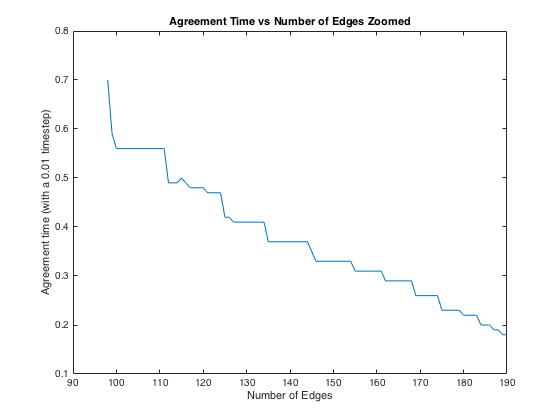
\includegraphics[width=\textwidth]{./Agreement_time-edges_zoomed.png}
\end{figure}
\begin{figure}[h!]
\caption{Second Eigenvalue}
\centering
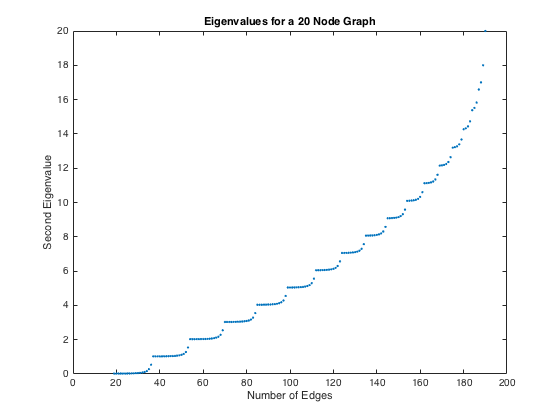
\includegraphics[width=\textwidth]{./Eigenvalues-edges.png}
\end{figure}


\section*{Bonus Question}
See \texttt{boids.tar.gz}. 




\end{document}
